\documentclass[conference]{IEEEtran}
\IEEEoverridecommandlockouts

\usepackage{cite}
\usepackage{amsmath,amssymb,amsfonts}
\usepackage{algorithmic}
\usepackage{graphicx}
\usepackage{textcomp}
\usepackage{xcolor}
\usepackage{booktabs}
\usepackage{multirow}
\usepackage{array}
\usepackage[
    colorlinks=true,
    linkcolor=blue,
    citecolor=blue,
    urlcolor=blue
]{hyperref}

\def\BibTeX{{\rm B\kern-.05em{\sc i\kern-.025em b}\kern-.08em
    T\kern-.1667em\lower.7ex\hbox{E}\kern-.125emX}}

\begin{document}

\title{Distributional Pedagogical Alignment:\\An Evidence-Centered Framework for Knowledge Tracing}

\author{%
\IEEEauthorblockN{Author One}
\IEEEauthorblockA{\textit{Department of Computer Science} \\
\textit{University Name}\\
City, Country \\
author1@university.edu}
\and
\IEEEauthorblockN{Author Two}
\IEEEauthorblockA{\textit{Department of Computer Science} \\
\textit{University Name}\\
City, Country \\
author2@university.edu}
}

\maketitle

\begin{abstract}
Knowledge Tracing (KT) models a learner's evolving knowledge state from historical interactions to predict future performance. Recent work on KT primarily targets richer interaction representations, distributional and uncertainty-aware knowledge states, and reasoning or interpretability mechanisms. We take an evidence-centered view of this task: an interaction supports a knowledge update only after it has been aggregated and interpreted under a pedagogical lens, and we treat this interpretation as an explicit intermediate stage rather than leaving it as an implicit update computation. We propose a framework organized into four representation spaces: Interaction, Distribution, Knowledge, and Prediction. At its core is the \emph{Distributional Pedagogical Alignment} module: interaction representations are projected into a distributional space, where learning patterns, which are structurally consistent across learners, are constructed and aligned with pedagogical principles, yielding the evidence that subsequently drives the knowledge-state update. This explicit stage also exposes an intrinsic, model-level attribution pathway from learning patterns to knowledge components to predictions, making these attributions available for inspection at the model level. This paper presents the framework and its rationale as a conceptual foundation for ongoing research on evidence-centered knowledge tracing.
\end{abstract}

\begin{IEEEkeywords}
Knowledge Tracing, Evidence-Centered Design, Learning Pattern, Distributional Representation, Pedagogical Alignment, Interpretability
\end{IEEEkeywords}

% ====================================================================
\section{Introduction}
\label{sec:intro}

Knowledge Tracing (KT) aims to model the evolving knowledge state of a learner from a history of learning interactions to predict the outcome of subsequent interactions~\cite{corbett1994kt, piech2015dkt}. Over the past years, KT models have advanced along a set of complementary directions: strengthening how interactions are represented (content-, topology-, and semantic-aware embeddings)~\cite{li2025mckt, xia2025cmdkt}; enriching how the knowledge state is represented (probabilistic or uncertainty-aware representations)~\cite{chen2025ukt, li2025keenkt, wu2026sskt}; and improving interpretability (graph, neural-symbolic, or probabilistic reasoning)~\cite{nakagawa2019gkt, zhou2024psikt, hooshyar2026nskt, wu2026plkt}. Each of these lines strengthens one facet of the same underlying task: turning a history of interactions into an estimate of what a learner knows. Educational measurement frames this task as inference from evidence: a learner's proficiency is not observed directly but must be inferred from observations, each carrying some ``weight and direction'' as evidence about that proficiency~\cite{mislevy2005ecd}. This view is reinforced by formative assessment, which treats each interaction as feedback that informs, rather than scores, a learner's developing understanding~\cite{black2009formative}. We take this evidence-centered view as the organizing principle of the framework, and use it to bring these complementary advances together rather than to set them against one another.

Following the evidence-centered view, we treat an interaction not as something that directly changes knowledge, but as a source of evidence that contributes to a knowledge update only after it has been aggregated and interpreted through a pedagogical lens. Most of the advances above act at the two ends of this process: how interactions are encoded and how outcomes are predicted, while the interpretation of the evidence in between is typically implicitly folded into the state update step. Our proposal is to give this interpretation a stage of its own.

Concretely, we introduce an explicit layer between the interaction representation and the mastery update, whose task is to interpret the evidence before it is used. This layer (i)~organizes interactions into \emph{learning patterns} that carry pedagogical meaning, (ii)~aligns those patterns with pedagogical principles, and (iii)~gives the evidence a structure that is consistent across learners. We organize the overall framework around this layer as four representation spaces: Interaction, Distribution, Knowledge, and Prediction, each intended to hold a single responsibility. Figure~\ref{fig:motivation} sketches these four spaces and locates the proposed layer among them.

\begin{figure}[!htbp]
\centering
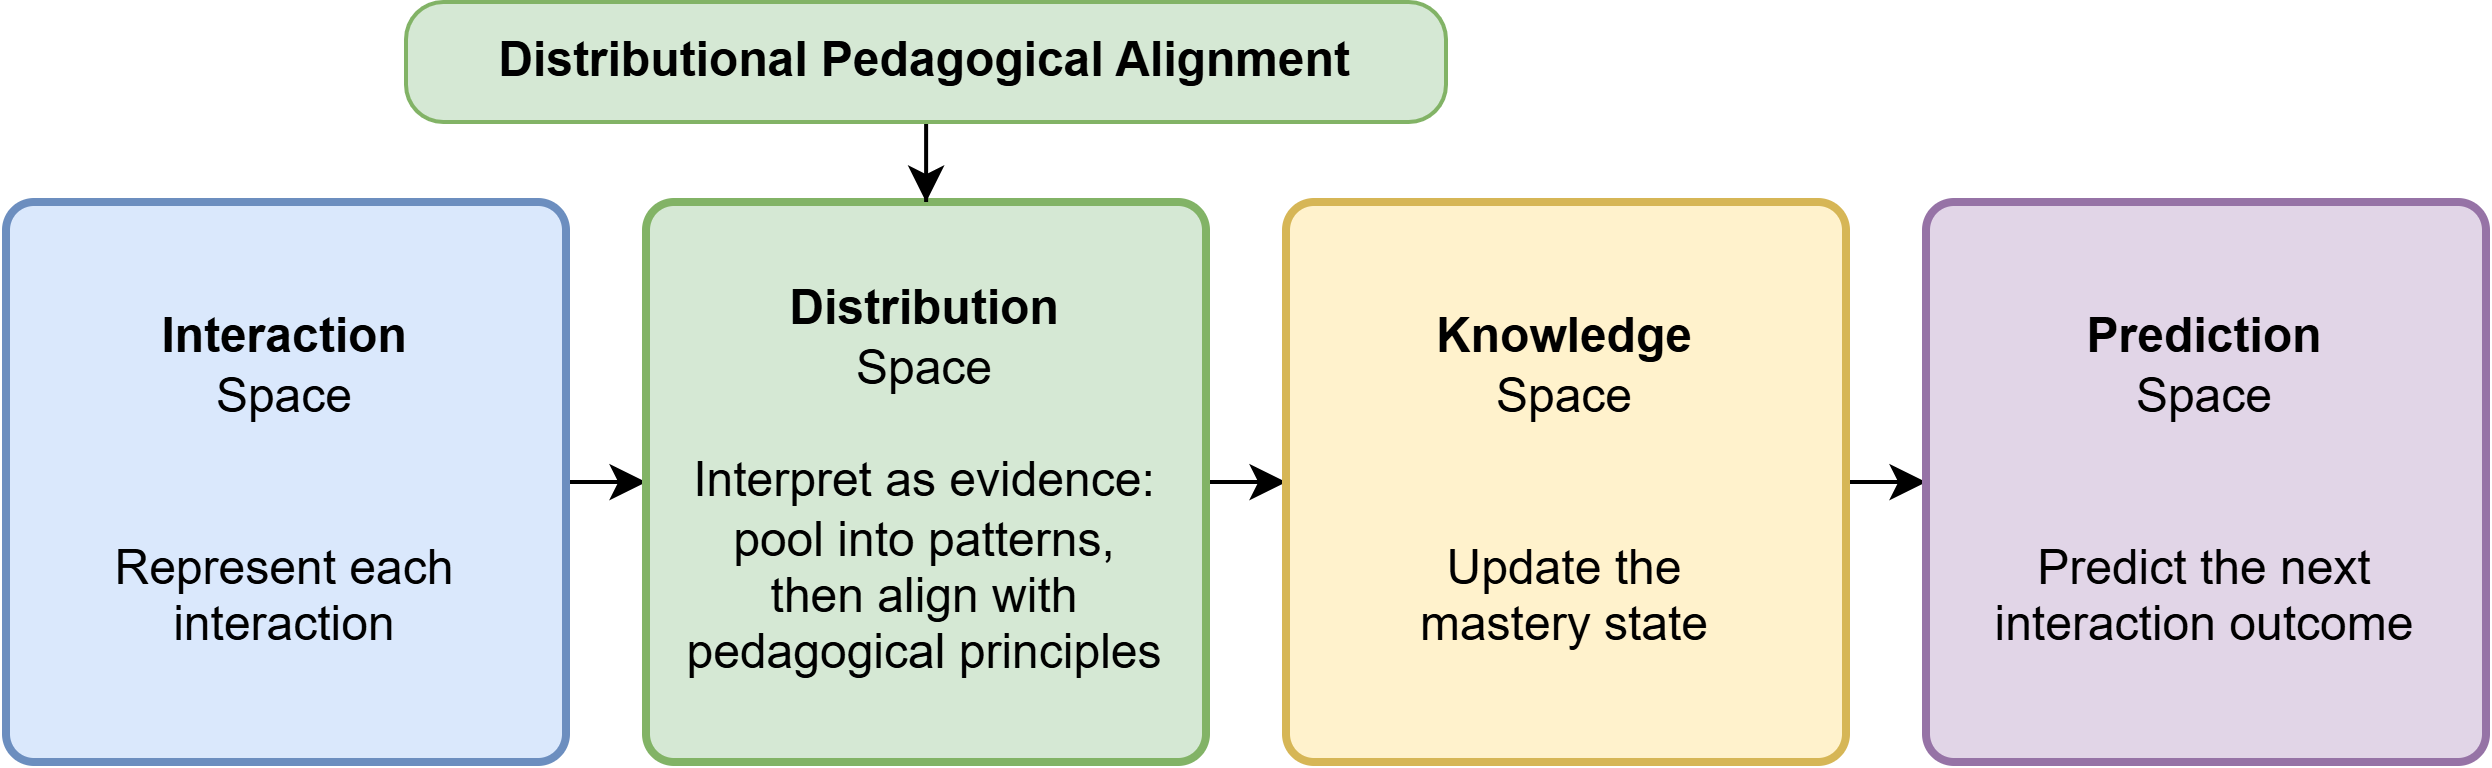
\includegraphics[width=\columnwidth]{designspace}
\caption{Design space of the proposed framework. Learner history flows through four representation spaces: Interaction, Distribution, Knowledge, and Prediction, each responsible for a different part of the process (with intermediate representations $z_t$, $z'$, $M_{t+1}$, and $\hat{y}$). The Distribution space hosts the proposed Distributional Pedagogical Alignment layer: an explicit evidence-interpretation stage, inserted between interaction representation and the mastery update, that pools interactions into learning patterns and aligns them with pedagogical principles.}
\label{fig:motivation}
\end{figure}

The contribution of this paper is threefold. First, a \emph{perspective}: it frames the knowledge update as an act of interpreting evidence, grounded in pedagogical theory. Second, a \emph{core mechanism}, Distributional Pedagogical Alignment, that gives this interpretation an explicit stage of its own, aligning learning patterns with pedagogical principles in a distributional space. Third, an \emph{architecture} that organizes the framework as four representation spaces. The explicit interpretation stage also exposes an intrinsic, model-level attribution trace. This trace opens a path toward interpretability, though it is yet, by itself, to guarantee a faithful explanation of the model's reasoning.

The rest of the paper is organized as follows. Section~\ref{sec:related} positions the framework in relation to recent KT research. Section~\ref{sec:formulation} formalizes the task and introduces notation. Section~\ref{sec:framework} presents the framework and its rationale, and Section~\ref{sec:discussion} discusses design choices and their implications. Section~\ref{sec:conclusion} concludes with a summary and an outlook on future work.

% ====================================================================
\section{Related Work and Positioning}
\label{sec:related}

Recent KT research can be read along three themes, which together offer complementary perspectives on how learner behavior can be modeled.

\textbf{Interaction representation.} The first theme enriches how interactions are encoded, drawing on question semantics, difficulty, and knowledge-component (KC) topology~\cite{li2025mckt, xia2025cmdkt}. These models improve the input to knowledge tracing without changing how the knowledge state itself is formed.

\textbf{Distributional and uncertainty-aware mastery.} The second theme represents the knowledge state, or the concepts themselves, as distributions and defines operations over them. For example, stochastic embeddings compared by an optimal-transport distance~\cite{chen2025ukt}, a Normal-Inverse-Gamma state shaped by a distributional contrastive objective~\cite{li2025keenkt}, and Gaussian KC embeddings propagated by a distributional distance~\cite{wu2026sskt}. This theme provides a vocabulary for expressing confidence and similarity that a point representation lacks.

\textbf{Reasoning and interpretability.} The third theme makes the inference more transparent through graph-based, probabilistic, or neural-symbolic reasoning~\cite{nakagawa2019gkt, zhou2024psikt, hooshyar2026nskt, wu2026plkt}, including pattern-based probabilistic embeddings that reason from evidence toward an outcome~\cite{wu2026plkt}. In particular, PLKT~\cite{wu2026plkt} is closest to our setting: it also reasons from patterns toward an outcome. Our framework differs in that the pattern comes from a latent that has already modeled the learner's history and is then aligned with pedagogical principles, rather than being assembled directly from raw interaction history.

Our framework connects to all three themes, each through a specific modeling choice. To represent an interaction, we enrich its encoding with knowledge-component topology, in the spirit of the first theme. To interpret the resulting evidence, we build learning patterns in a distributional space, drawing on the second theme's distributional vocabulary but putting it to pedagogical use. And to adjust those patterns, we align them with pedagogical principles through a soft, principle-guided mechanism, echoing the third theme's use of structured reasoning while keeping the adjustment soft rather than deductive. The distinctive element is this last step: a layer that aligns learning patterns, structured consistently across learners, with pedagogical principles prior to knowledge state update. We treat the works above as alternative design choices for related components rather than as baselines to outperform; where a choice differs from ours, we discuss it alongside our own in Sections~\ref{sec:framework} and~\ref{sec:discussion}.

% ====================================================================
\section{Problem Formulation and Notation}
\label{sec:formulation}

A learner's interaction history is a sequence $S_t=\{(q_t, r_t)\}_{t=1}^{T}$, where $q_t$ is the question (item) attempted at step $t$ and $r_t \in \{0,1\}$ indicates an incorrect/correct response. The KT task is to predict $P(r_{t+1}=1 \mid q_{t+1}, S_t)$. The domain's knowledge structure is a set of knowledge components (KCs) $\mathcal{C}=\{c_1,\dots,c_C\}$, a question-to-KC mapping, and a knowledge graph $\mathcal{G}$ encoding heterogeneous relations (e.g., prerequisite, neighboring, applying) among KCs. Within the scope of this paper, we treat $\mathcal{G}$ as a given, validated input (Section~\ref{sec:disc-kg}).

The framework threads a learner's history through four representation spaces. We keep the notation at the level needed to describe the flow and leave the transformation equations to our future implementation paper.

\begin{table}[!htbp]
\caption{Notation used throughout the paper.}
\label{tab:notation}
\centering
\renewcommand{\arraystretch}{1.25}
\begin{tabular}{@{}p{0.11\columnwidth}p{0.20\columnwidth}p{0.56\columnwidth}@{}}
\toprule
\textbf{Symbol} & \textbf{Space} & \textbf{Meaning} \\
\midrule
$z_t$ & Interaction & Interaction representation at step $t$ (fused context). \\
$h_t$ & Distribution & Distributional representation at step $t$, given by statistical descriptors. \\
$P_i,\tilde{P}_i$ & Distribution & Learning pattern from operator $i$, before and after alignment. \\
$z'$ & Distribution & Structured pattern representation (readout); this post-alignment object is what we call \emph{evidence}. \\
$M_t$ & Knowledge & Explicit mastery state before the update at step $t$. \\
$A_i$ & Knowledge & Contribution of pattern $i$ onto related KCs. \\
$W$ & Prediction & Contribution of each KC onto the target prediction. \\
$\hat{y}$ & Prediction & Predicted probability of a correct response to $q_{t+1}$. \\
\bottomrule
\end{tabular}
\end{table}

\noindent\textbf{Terminology.} We use \emph{evidence} for the distributional representation in the alignment layer \emph{after} it has been pooled into patterns and pedagogically adjusted: a post-alignment object. A \emph{learning pattern} is the output of a fixed aggregation operator, defined by the aggregation rather than by the number of interactions it draws on.

% ====================================================================
\section{Proposed Framework}
\label{sec:framework}

\begin{figure*}[!t]
\centering
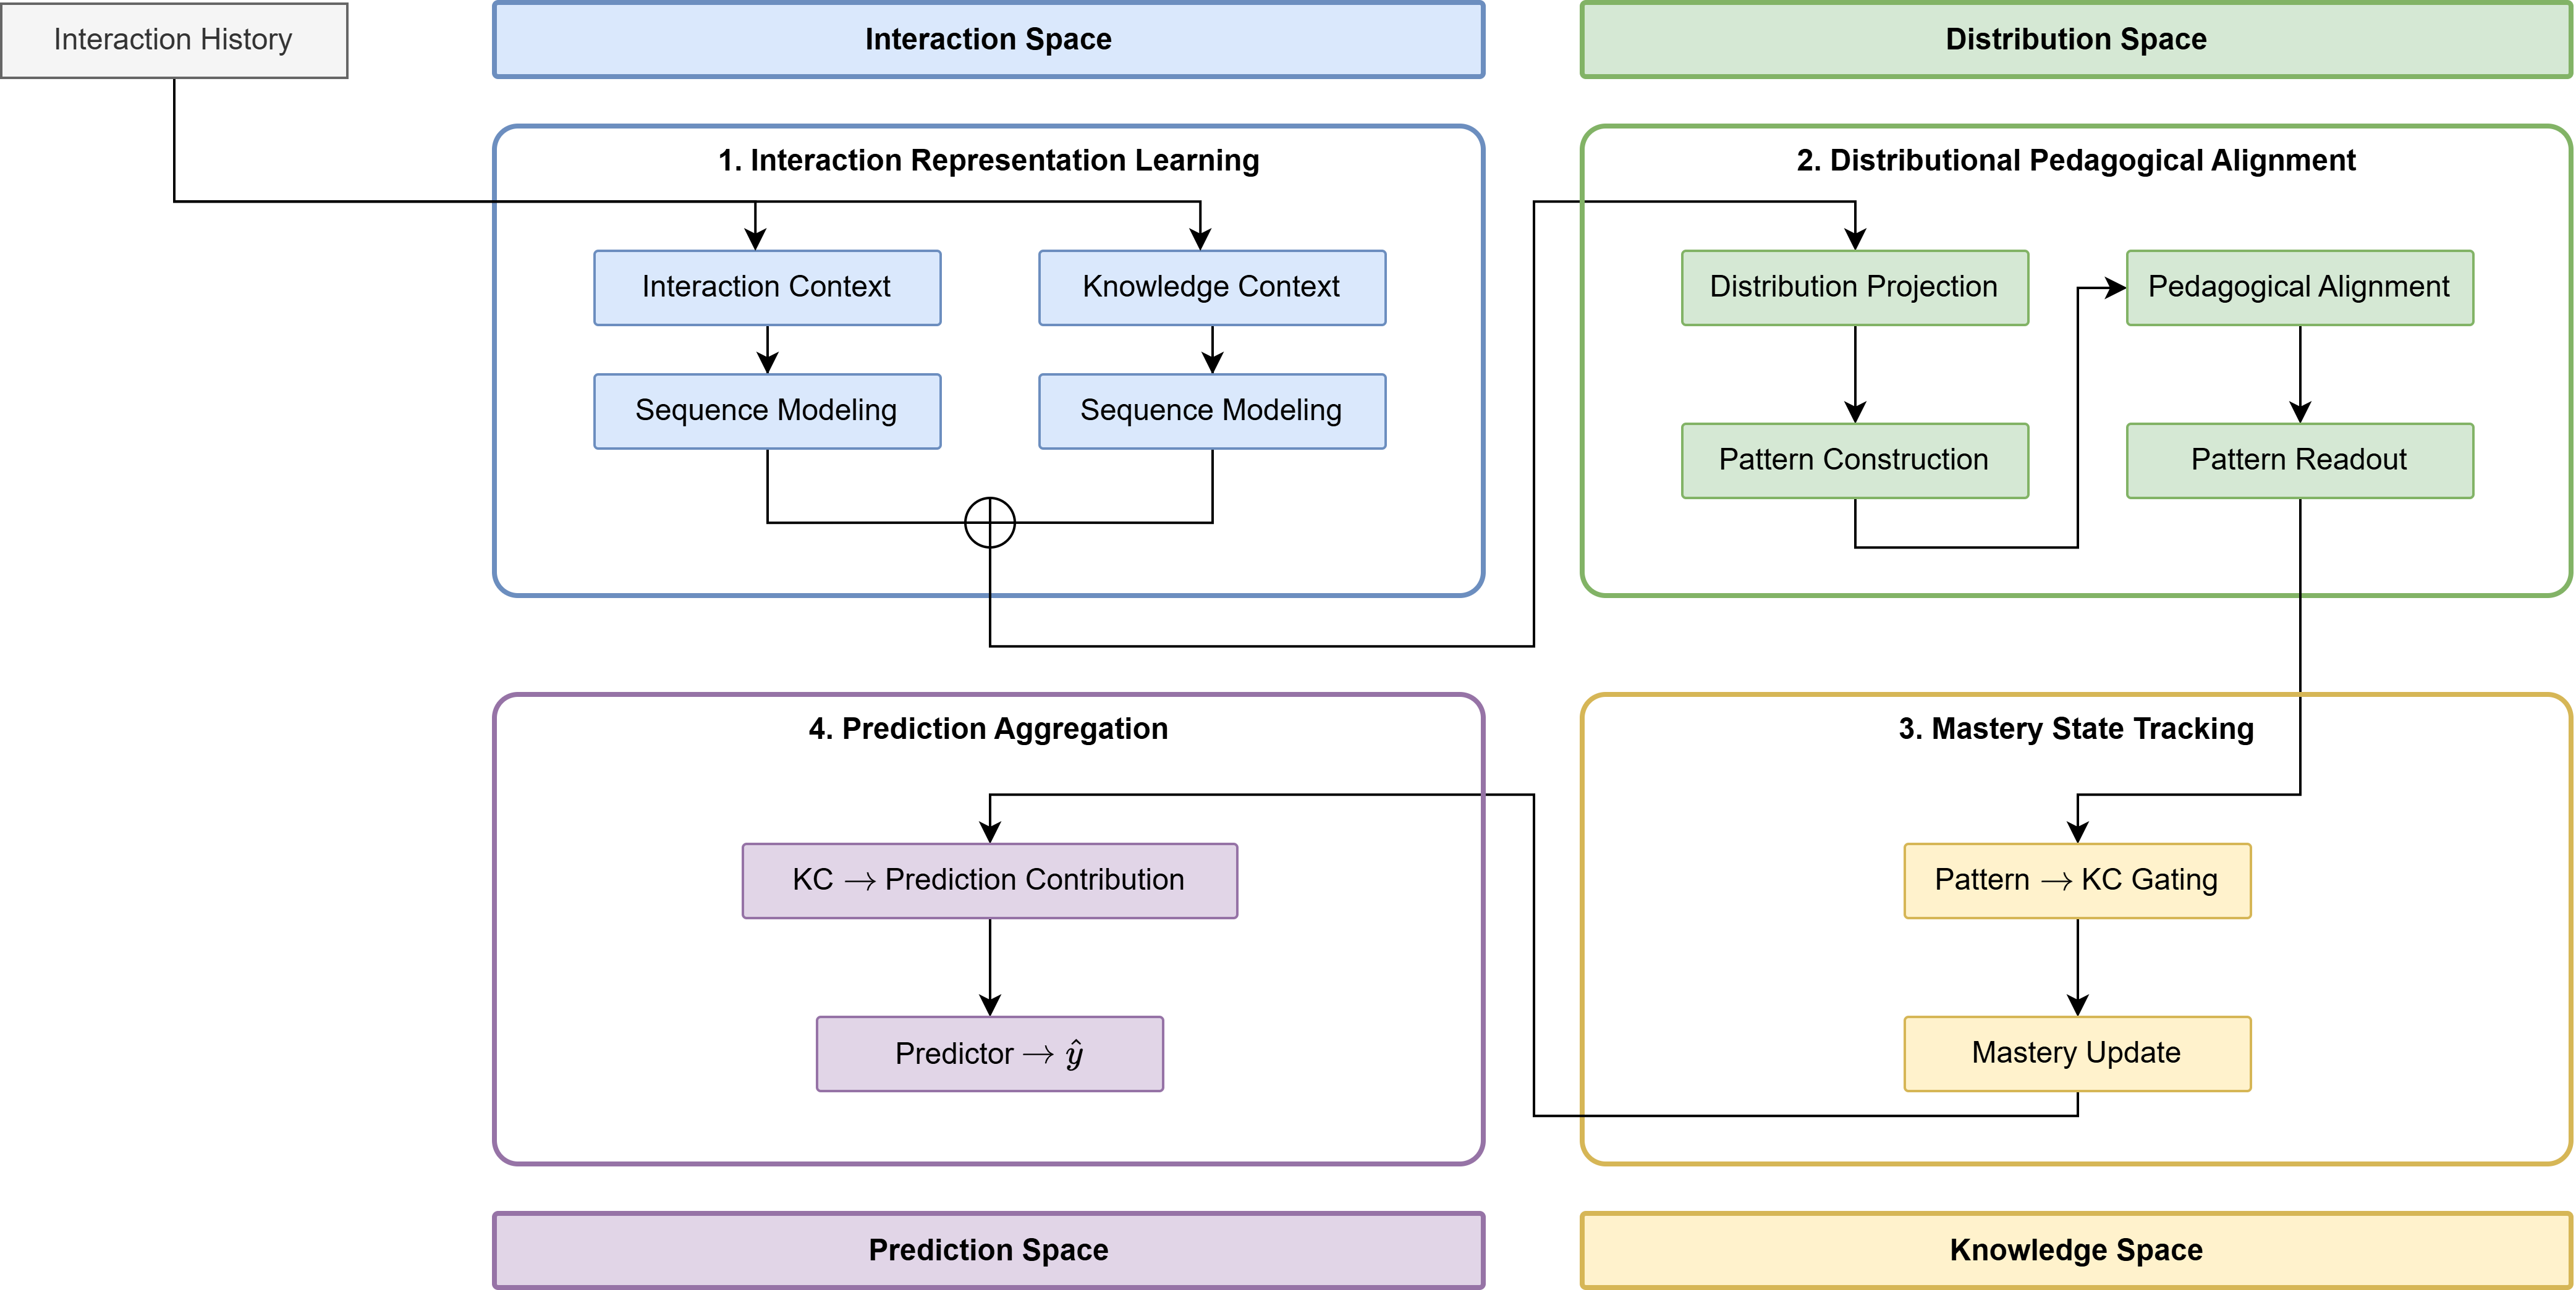
\includegraphics[width=0.92\textwidth]{framework}
\caption{Framework overview. Four modules over four representation spaces (color-coded). Evidence is \emph{produced} in Module~2, the mastery state is \emph{updated} in Module~3, and the prediction is formed in Module~4. The dashed ribbon shows the intrinsic, model-level attribution trace the architecture exposes: interactions $\rightarrow$ learning patterns $\rightarrow$ pattern-to-KC contribution ($A_i$) $\rightarrow$ mastery/knowledge state $\rightarrow$ KC-to-prediction contribution ($W$) $\rightarrow$ prediction.}
\label{fig:framework}
\end{figure*}

\subsection{Design Rationale and Perspective}
\label{sec:rationale}

The framework realizes the sequence \emph{interaction $\rightarrow$ evidence $\rightarrow$ aggregation and adjustment $\rightarrow$ update}, with a separation of roles across the four spaces: each space pursues a single objective, keeping context, knowledge, and prediction from being mixed into a single representation. We treat this separation as a design aim. Mechanisms that encourage it, such as per-module contrastive objectives, which are precedent in KT~\cite{li2025keenkt}, are natural to add at implementation time.

\subsection{Overview}

The framework comprises four sequential modules, mapped one-to-one onto the four spaces (Figure~\ref{fig:framework}). Module~1 learns the interaction representation $z_t$. Module~2 turns $z_t$ into a distributional representation, pools it into learning patterns, aligns them with pedagogical principles, and reads out the structured evidence $z'$. Module~3 updates the explicit knowledge state $M_{t+1}$ from $z'$ while learning a pattern-to-KC contribution. Module~4 aggregates $M_{t+1}$ with the target question to produce $\hat{y}$ and a KC-to-prediction contribution.

\subsection{Module 1: Interaction Representation Learning}
\label{sec:irl}

The first module learns a contextual representation for each interaction from two input groups with distinct learning dynamics. The \emph{interaction context} gathers question semantics, the student response, and question difficulty. The \emph{knowledge context} combines a localized mastery representation with concept difficulty; localized mastery is obtained by reading the mastery memory in the context of the current question via the knowledge graph. The two groups are processed by two parallel sequence-modeling branches: one capturing the dynamics of the interaction sequence, the other the dynamics of the local knowledge state. The two representations are fused into $z_t$.

\subsection{Module 2: Distributional Pedagogical Alignment}
\label{sec:dpa}

The alignment layer proceeds in four conceptual steps:

\begin{enumerate}
    \item~\emph{Distribution projection} maps $z_t$ to a distributional representation $h_t$ via a statistical-descriptor decoder. The distributional space is an \emph{intermediate representation space for interaction patterns}.
    \item~\emph{Pattern construction} builds several learning patterns using fixed pattern operators, so that each operator always carries the same pedagogical meaning and pattern structure is consistent across all learners regardless of history length or distribution. An open list of operators is: (i)~temporal pooling, which pools the most recent $k$ interactions; (ii)~same-KC pooling, which pools all interactions on the same KC; (iii)~prerequisite pooling, which pools all interactions on prerequisite KCs; and (iv)~neighbor-concept pooling, which pools all interactions on neighboring KCs.
    \item~\emph{Pedagogical alignment} aligns the patterns with pedagogical principles. Crucially, this adjustment does not directly infer mastery; instead, it nudges the patterns toward those principles, serving as a soft (differentiable) regularization over the distributional space rather than a hard deductive rule. An open list of principles is: (i)~\emph{guessing and slipping}, which adjusts a pattern to allow a correct response despite low mastery (guessing) or an incorrect response despite high mastery (slipping); and (ii)~\emph{monotonicity}, which discourages unwarranted drops in mastery when the evidence is consistent with continued learning.
    \item~\emph{Pattern readout} maps the aligned patterns back to a structured vector $z'$, in which each block corresponds to one pattern type.
\end{enumerate}

\smallskip
\noindent\textbf{Reasoning for distributional space.} Representing patterns as distributions rather than plain vectors serves the two operations of this layer. Pooling preserves both location and dispersion, so a pattern retains a sense of how concentrated its supporting evidence is, and the pedagogical distance between two patterns can be expressed as a divergence with a defined meaning. The space is used here specifically for pedagogical pattern-pooling and alignment; we discuss its role further in Section~\ref{sec:disc-dist}.

\subsection{Module 3: Mastery State Tracking}
\label{sec:mst}

The third module maintains an explicit knowledge state $M_t$ and updates it from the structured pattern representation $z'$. Alongside the update, it learns a \emph{pattern-to-KC gating} $A_i = G(P_i)$ that quantifies how much each learning pattern contributes to each related KC, and the state advances by a residual increment.

The gating makes it possible to ask which learning pattern raised the mastery of a given KC; we return to how far such readings can be interpreted in Section~\ref{sec:interp}.

\subsection{Module 4: Prediction Aggregation}
\label{sec:pred}

The final module predicts the outcome of the next interaction from the updated knowledge state $M_{t+1}$ and a representation of the target question $q_{t+1}$. Alongside the probability, it produces a \emph{KC contribution} $W = C(M_{t+1}, q_{t+1})$ (contribution of each KC to the target interaction) and forms the prediction $\hat{y} = f(M_{t+1}, q_{t+1}, W)$.

\subsection{Intrinsic Interpretability: Attribution Trace}
\label{sec:interp}

Combining the pattern-to-KC gating of Module~3 (\ref{sec:mst}) with the KC-to-prediction contribution of Module~4 (\ref{sec:pred}) yields a single attribution trace that runs through the whole model: historical interactions $\rightarrow$ learning patterns $\rightarrow$ pattern-to-knowledge contribution $\rightarrow$ updated knowledge state $\rightarrow$ knowledge-to-prediction contribution $\rightarrow$ prediction (dashed ribbon, Figure~\ref{fig:framework}). These attributions are derived from the model's own computation rather than from a separate post hoc explainer. The framework thus supports the extraction of model-level attributions that help explain how a prediction was formed. Whether such weights are faithful accounts of the model's reasoning is a known question in prior work~\cite{jain2019attention,wiegreffe2019attention}. Evaluation of such faithfulness is part of our planned work.

% ====================================================================
\section{Discussion}
\label{sec:discussion}

\subsection{Role of the Distributional Space}
\label{sec:disc-dist}

The distributional space plays a specific role in the framework: it is where evidence is pooled into patterns and aligned. Both operations are natural over distributions: pooling carries location and dispersion together, so a pattern retains a sense of how concentrated the underlying evidence is, and pedagogical distance between patterns can be expressed as a divergence with a defined meaning. A further consequence of our design is where the distribution originates: because it is interpreted from a latent that has already modeled the history rather than read from raw interactions, the resulting representation reflects the model's current understanding of the learner. Distributional representations are indeed established in the literature~\cite{chen2025ukt, li2025keenkt, wu2026sskt}; the particular here is using the space for pedagogical pattern construction and alignment.

\subsection{Knowledge Graph as Structural Input}
\label{sec:disc-kg}

The prerequisite and neighbor operators read from a knowledge graph that the framework takes as structural input. Such graphs can be obtained reliably in practice; for instance, \texttt{CMDKT}~\cite{xia2025cmdkt} generates prerequisite relations with a language model and validates them with domain experts, and we assume a graph prepared in this manner. A natural extension is to learn the topology itself, as in approaches that infer KC relations when explicit annotations are unavailable~\cite{wu2026sskt}; we see this as a promising direction to combine with the present design.

\subsection{Nature of the Pedagogical Adjustment}
\label{sec:disc-soft}

The alignment layer adjusts patterns by aligning them with pedagogical principles, rather than by applying hard deductive rules that infer mastery directly (as in neural-symbolic approaches~\cite{hooshyar2026nskt}) or by leaving the adjustment entirely to be learned. This alignment keeps a pedagogical prior in the model while leaving room for the data to shape the representation.

% ====================================================================
\section{Conclusion}
\label{sec:conclusion}

We have presented a perspective on knowledge tracing in which updating knowledge is the interpretation of evidence, realized through an explicit intermediate layer, Distributional Pedagogical Alignment, that pools interactions into learning patterns whose structure is consistent across learners and aligns them with pedagogical principles prior to mastery update. The framework's central addition is exactly this pedagogical alignment of learning patterns, together with an intrinsic, model-level attribution trace that the architecture exposes. As an ongoing research effort, our immediate research goals are to implement the framework and evaluate it on standard benchmarks; to study mechanisms that encourage the intended role separation; to evaluate the faithfulness of the attribution trace; and to relax the knowledge graph toward a learnable topology.

% ====================================================================
% References
% ====================================================================
\bibliographystyle{IEEEtran}
\bibliography{references}

\end{document}
